%To compile as handout, use
%pdflatex "\def\ishandout{1} \input{filename.tex}"
%Defaults to non-handout mode (with slide reveals)
\ifdefined\ishandout
  \documentclass[handout]{beamer}
\else
  \documentclass{beamer}
\fi
 
\usepackage{econ103slides} 

\date{Lecture 20}


\begin{document} 




%%%%%%%%%%%%%%%%%%%%%%%%%%%%%%%%%%%%%%%%

\begin{frame}[plain]
	\titlepage 
	

\end{frame} 

%%%%%%%%%%%%%%%%%%%%%%%%%%%%%%%%%%%%%%%%
\begin{frame}
\begin{center}
\Huge Hypothesis Testing II
\end{center}
\end{frame}

%%%%%%%%%%%%%%%%%%%%%%%%%%%%%%%%%%%%%%%%
\begin{frame}
	\frametitle{What if the null is false?}

	\begin{block}
		{Alternative hypothesis: $H_1$}
		The \emph{negation} of the null hypothesis.
	\end{block}
	\begin{block}
		{Examples:}
		\begin{enumerate}
			\item 
				\begin{itemize}
					\item $H_0\colon$ This parameter equals 5.
				\item $H_1\colon$ This parameter does \emph{not} equal 5.
		\end{itemize}
			\item 
				\begin{itemize}
					\item $H_0\colon$ There is no difference between these two groups.
					\item $H_1\colon$ There \emph{is} a difference between these two groups.
				\end{itemize}
		\end{enumerate}
		
	\end{block}

	\alert{Sometimes we only care about \emph{certain kinds} of violations of $H_0$...}
\end{frame}
%%%%%%%%%%%%%%%%%%%%%%%%%%%%%%%%%%%%%%%%
\begin{frame}
\frametitle{One-sided vs.\ Two-sided Alternative}
\alert{Let $\theta$ be a population parameter and $\theta_0$ be a specified constant.}
\begin{block}
	{Null Hypothesis}
\begin{itemize}
	\item $H_0\colon \theta = \theta_0$
\end{itemize}\end{block}
	\begin{block}{Two-sided Alternative}
		\begin{itemize}
			\item $H_1\colon \theta \neq \theta_0$
		\end{itemize}
\end{block}
	\begin{block}{One-sided Alternative}
		Two possibilities, depending on the problem at hand:
		\begin{itemize}
			\item $H_1\colon \theta > \theta_0$
			\item $H_1\colon \theta < \theta_0$
		\end{itemize}
\end{block}
\end{frame}

%%%%%%%%%%%%%%%%%%%%%%%%%%%%%%%%%%%%%%%%
\begin{frame}
\frametitle{Example: Suing McDonald's \hfill 
\includegraphics[scale = 0.05]{./images/clicker}}

A class action lawsuit claims that McDonald's has been  understating the caloric content of the ``Big Mac,'' misleading consumers into thinking the sandwich is healthier than it really is. McDonald's claims the sandwich contains $550$ kcal on average. \\

\vspace{1em}
\alert{Suppose you're the judge in this case. What is your alternative hypothesis?}

	\begin{enumerate}[(a)]
		\item $H_1\colon \mu \neq 550$ kcal
		\item $H_1\colon \mu < 550$ kcal
		\item $H_1\colon \mu > 550$ kcal
		\item $H_1\colon \mu = 550$ kcal
\end{enumerate}
\end{frame}
%%%%%%%%%%%%%%%%%%%%%%%%%%%%%%%%%%%%%%%%

\begin{frame}
\frametitle{Example: Quality Control at McDonald's \hfill 
\includegraphics[scale = 0.05]{./images/clicker}}

You are a senior manager at McDonald's and are concerned that franchises may be deviating from company policy on the calorie count of a Big Mac sandwich, which is supposed to be 550 kcal on average. Because intervening is costly, you will only take action is there is strong evidence of deviation from company policy. \\

\vspace{1em}

\alert{What is your alternative hypothesis?}
	\begin{enumerate}[(a)]
		\item $H_1\colon \mu \neq 550$ kcal
		\item $H_1\colon \mu < 550$ kcal
		\item $H_1\colon \mu > 550$ kcal
		\item $H_1\colon \mu = 550$ kcal
\end{enumerate}
\end{frame}
%%%%%%%%%%%%%%%%%%%%%%%%%%%%%%%%%%%%%%%%%
\begin{frame}
	\frametitle{Decision Rule: When should we reject $H_0$?}
	\begin{itemize}
		\item Test statistic: RV with known sampling distribution under $H_0$
		\item McDonald's Example: $T_n = 3(\bar{X} - 550)/S$
		\item \emph{Random} since $\bar{X}$ and $S$ are RVs under random sampling: functions of $X_1, \hdots, X_9$.
		\item Observed dataset: \emph{realizations} $x_1, \hdots, x_9$ of RVs $X_1, \hdots, X_9$
		\item Plug in observed data to get estimates (constants) $\bar{x}$ and $s$.
		\item Plug these into the formula for the test statistic to get a \emph{number} -- this is a \emph{realization} of $T_n$ 
		\item Depending on this number, decide whether to reject $H_0$.
	\end{itemize}
\end{frame}
%%%%%%%%%%%%%%%%%%%%%%%%%%%%%%%%%%%%%%%%%
\begin{frame}
\frametitle{What Form Should the Decision Rule Take?}
\begin{columns}
\begin{column}{6cm}
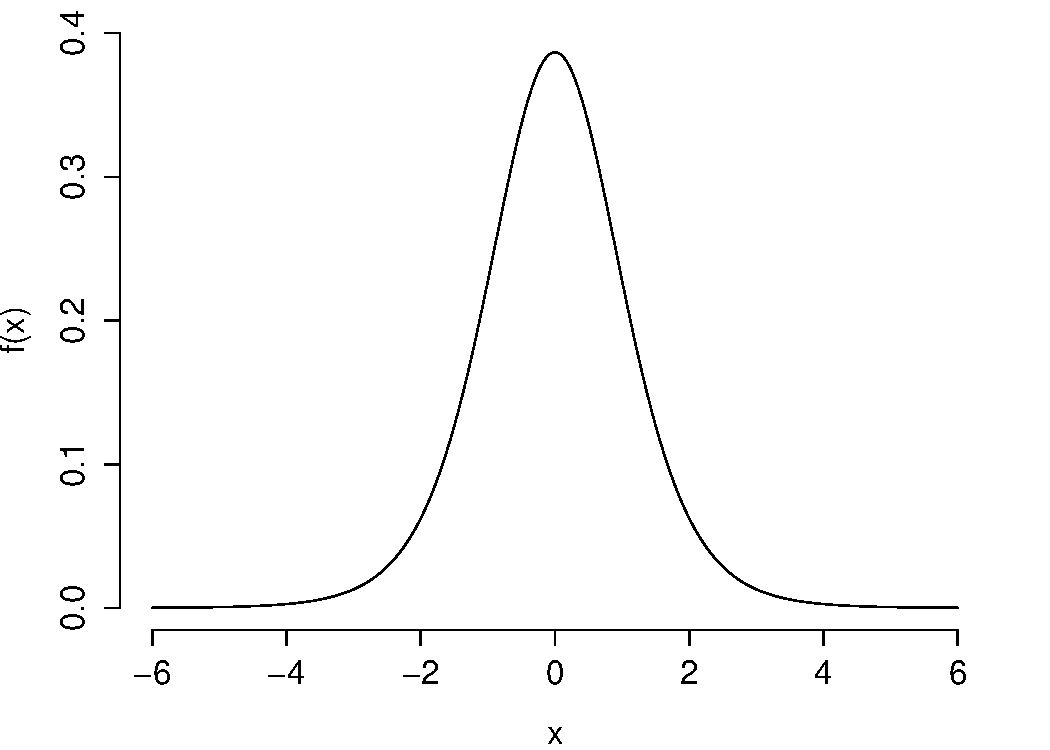
\includegraphics[scale = 0.5]{./images/t_pdf}
\end{column}

\begin{column}{6cm}
$H_0\colon \mu=550 \Rightarrow \displaystyle \frac{\bar{X} - 550}{S/3} \sim t(8)$\\ \pause
\vspace{1em}
One-sided Alternative $H_1\colon \mu > 550$\\ \pause
\vspace{1em}
Two-sided Alternative $H_1\colon \mu \neq 550$ 
\end{column}

\end{columns}
 
\end{frame}
%%%%%%%%%%%%%%%%%%%%%%%%%%%%%%%%%%%%%%%%
\begin{frame}
\frametitle{Example: Suing McDonald's \hfill 
\includegraphics[scale = 0.05]{./images/clicker}}
The plaintiffs allege that McDonald's has \emph{understated} the true caloric content of a Big Mac: it's actually \emph{greater} than 550 kcal. \alert{Suppose the plaintiffs are right. Then what sort of value should we expect the test statistic $3(\bar{X} - 550)/S$ to take on?}

\vspace{1em}
\begin{enumerate}[(a)]
	\item A value \emph{less} than zero.
	\item A value close to zero.
	\item A value \emph{greater} than zero.
\end{enumerate}
\end{frame}
%%%%%%%%%%%%%%%%%%%%%%%%%%%%%%%%%%%%%%%%
\begin{frame}
\frametitle{Example: Quality Control at McDonald's \hfill 
\includegraphics[scale = 0.05]{./images/clicker}}
The senior manager is worried that franchises are deviating from company policy that Big Macs should contain approximately 550 kcal. \alert{If the franchises \emph{are} deviating, what sort of of value should we expect the test statistic $3(\bar{X} - 550)/S$ to take on?}

\vspace{1em}
\begin{enumerate}[(a)]
	\item A value \emph{less} than zero.
	\item A value close to zero.
	\item A value \emph{greater} than zero.
	\item A value different from zero but we can't tell whether it will be positive or negative.
\end{enumerate}
\end{frame}
%%%%%%%%%%%%%%%%%%%%%%%%%%%%%%%%%%%%%%%%
\begin{frame}
\frametitle{What Form Should the Decision Rule Take?}
$X_1, \hdots, X_n \sim \mbox{iid } N(\mu, \sigma^2)$ 
\begin{block}{Common Null Hypothesis $H_0\colon \mu = 550$}
Under $H_0$, $T_n = \sqrt{n}(\bar{X}_n - 550)/S \sim t(n-1)$ 
\end{block}
\begin{block}{One-sided Alternative $H_1\colon \mu > 550$}
Reject $H_0$ if $T_n$ is ``too big'' 
\end{block}
\begin{block}{Two-sided Alternative $H_1\colon \mu \neq 550$} 
Reject $H_0$ if $T_n$ is ``too big'' or ``too small''
\end{block}

\vspace{1em}

\alert{But how big of a discrepancy is ``big enough'' to reject?}
\end{frame}

%%%%%%%%%%%%%%%%%%%%%%%%%%%%%%%%%%%%%%%%
\begin{frame}
	\frametitle{Two Kinds of Mistakes in Hypothesis Testing}
	\begin{block}
		{Type I Error}
		\begin{itemize}
			\item Rejecting the null when it's actually true.
			\item $P(\mbox{Type I Error}) = \alpha\quad \quad$ 
			\alert{$\boxed{\alpha= \mbox{``Significance Level'' of Test}}$}
		\end{itemize}
	\end{block}
	 \begin{block}
		{Type II Error}
		\begin{itemize}
			\item Failing to reject the null when it's false.
			\item $P(\mbox{Type II Error}) = \beta \quad \quad$ 
			\alert{$\boxed{1 - \beta= \mbox{``Power'' of Test}}$}
		\end{itemize}
	\end{block}
	\begin{alertblock}
		{Important!}
		Hypothesis testing \emph{controls} probability of a Type I error since this is assumed to be the \emph{worse} kind of mistake: convicting the innocent.	
	\end{alertblock}
\end{frame}
%%%%%%%%%%%%%%%%%%%%%%%%%%%%%%%%%%%%%%%%%
\begin{frame}
	\frametitle{Construct a Decision Rule to \emph{Fix} $\alpha$ at User-Chosen Level}

	\begin{block}
		{Critical Value $c_{\alpha}$} 
	\begin{itemize}
		\item Threshold for rejecting $H_0$
		\item Chosen so that $P(\mbox{Reject } H_0|H_0 \mbox{ is True}) = \alpha$
		\item Depends on \emph{both} $\alpha$ \emph{and} the alternative hypothesis.
	\end{itemize}
	\end{block}
	\begin{block}
		{One-Sided Alternative}
		Reject $H_0$ if $T_n >$ Critical Value
	\end{block}
	\begin{block}
		{Two-Sided Alternative}
		Reject $H_0$ if $|T_n| >$ Critical Value
	\end{block}
\end{frame}
%%%%%%%%%%%%%%%%%%%%%%%%%%%%%%%%%%%%%%%%%
\begin{frame}
\frametitle{Example: One-sided Alternative $H_1\colon \mu > 550$}
The critical value is chosen to reflect both the alternative hypothesis and the significance level. 
\begin{figure}
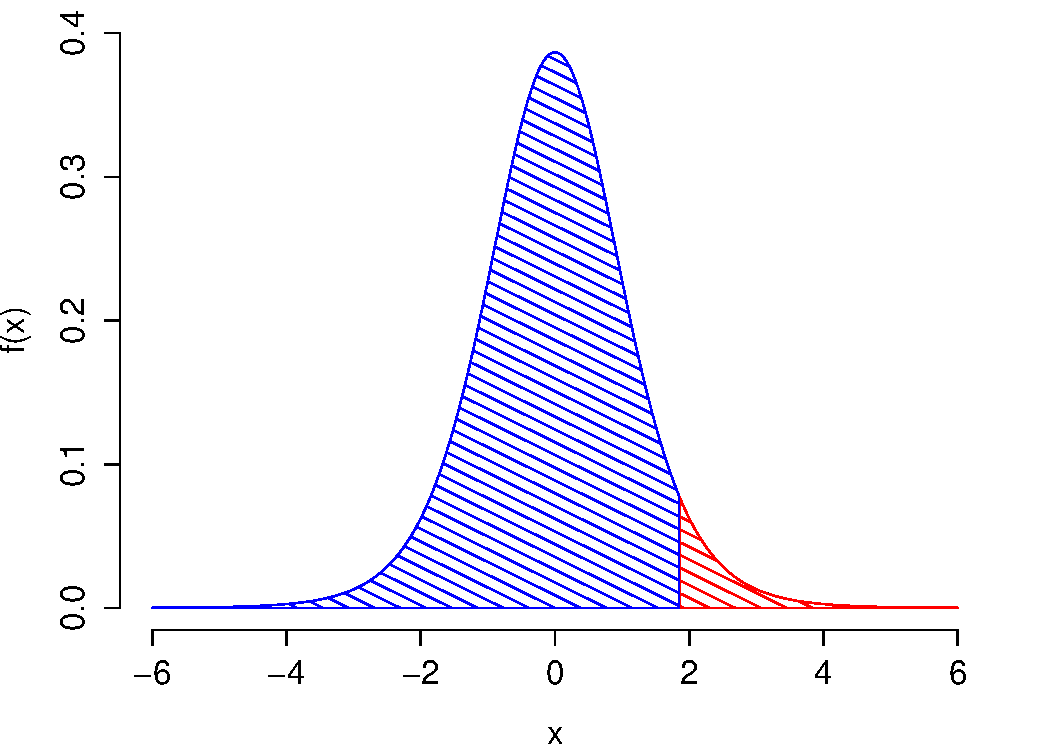
\includegraphics[scale = 0.45]{./images/one_side}
\end{figure}
One-sided Critical Value: \texttt{qt($1-\alpha$, df  = $n-1$)}
\end{frame}


%%%%%%%%%%%%%%%%%%%%%%%%%%%%%%%%%%%%%%%%

\begin{frame}
\frametitle{Example: Two-sided Alternative $H_1\colon \mu \neq 550$}
The critical value is chosen to reflect both the alternative hypothesis and the significance level. 
\begin{figure}
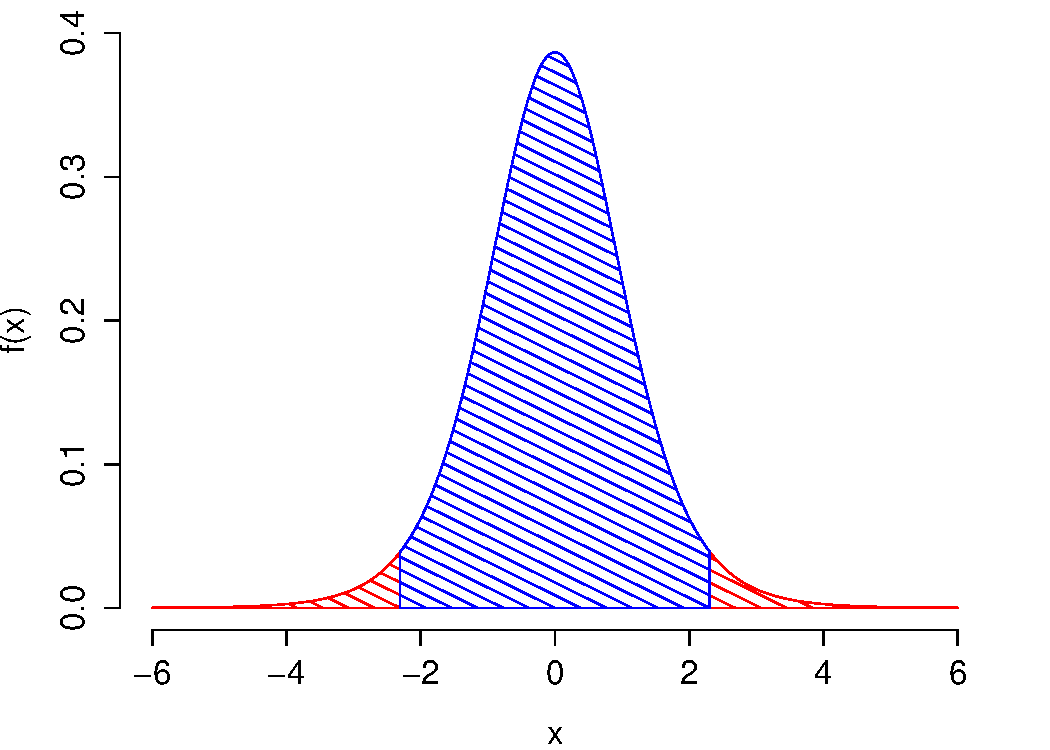
\includegraphics[scale = 0.45]{./images/two_side}
\end{figure}
Two-sided Critical Value: \texttt{qt($1-\alpha/2$, df  = $n-1$)}
\end{frame}

%%%%%%%%%%%%%%%%%%%%%%%%%%%%%%%%%%%%%%%%
\begin{frame}
Suppose, for example, $\alpha = 0.05$, $n = 9$
	\begin{eqnarray*}
		&&\texttt{qt(0.95, df  = 8)}\approx 1.86\\
		 &&\texttt{qt(0.975, df  = 8)}\approx 2.3
	\end{eqnarray*}
\begin{figure}
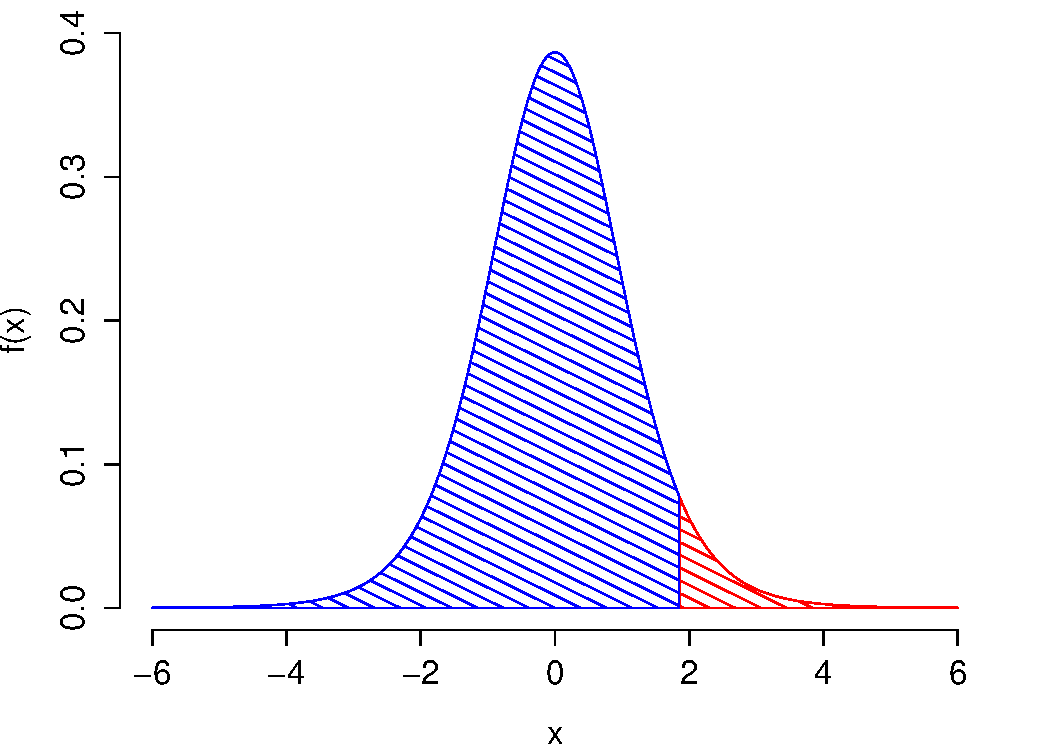
\includegraphics[scale = 0.3]{./images/one_side}
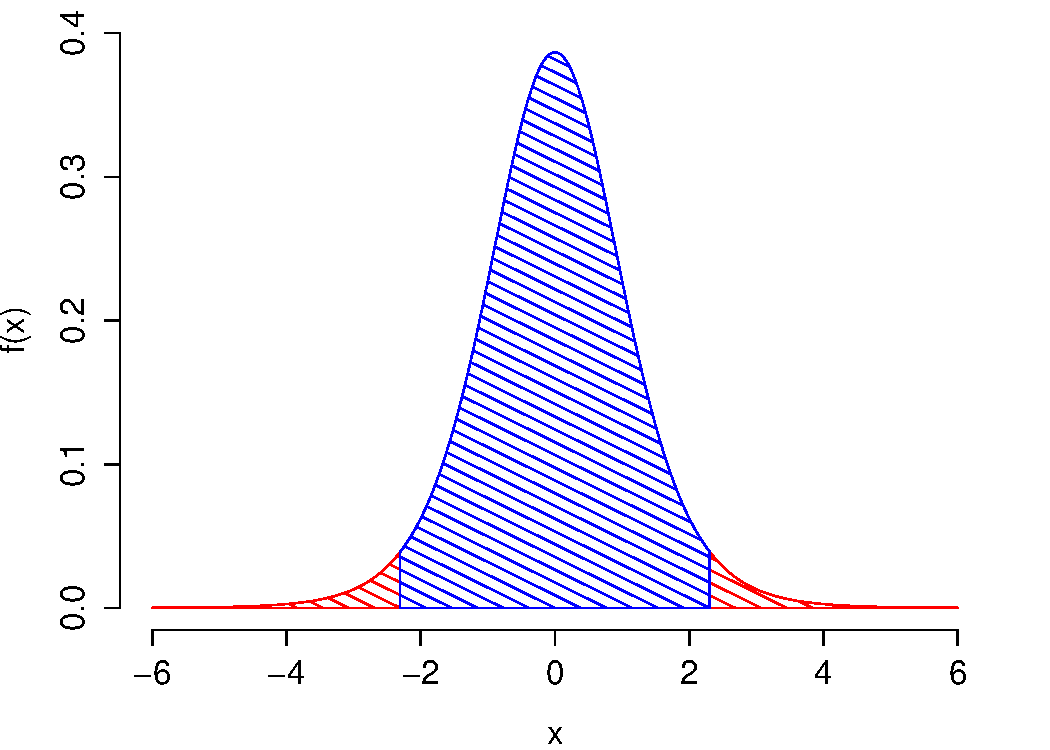
\includegraphics[scale = 0.3]{./images/two_side}
\end{figure}
One-sided Alternative: Reject $H_0$ if $3(\bar{X}_n - 550)/S \geq 1.86$\\
\vspace{0.5em}
Two-sided Alternative: Reject $H_0$ if $\left|3(\bar{X}_n - 550)/S\right| \geq 2.3$\\

\end{frame}

%%%%%%%%%%%%%%%%%%%%%%%%%%%%%%%%%%%%%%%%
\begin{frame}
\frametitle{McDonald's Example\hfill 
\includegraphics[scale = 0.05]{./images/clicker}}
Suppose $n=9$, $\bar{x} = 563$, $s = 34$. What is  the value of our test statistic?

\pause
\vspace{1em}
	$$\frac{563 - 550}{34/\sqrt{9}}= \frac{13}{34/3} \approx 1.14$$


\end{frame}

%%%%%%%%%%%%%%%%%%%%%%%%%%%%%%%%%%%%%%%%
\begin{frame}[t]
\frametitle{McDonald's Example: $\alpha = 0.05$\hfill 
\includegraphics[scale = 0.05]{./images/clicker}}
Recall that:
\begin{eqnarray*}
		&&\texttt{qt(0.95, df  = 8)}\approx 1.86\\
		 &&\texttt{qt(0.975, df  = 8)}\approx 2.3
	\end{eqnarray*}
Based on an observed test statistic of $1.14$, would we reject $H_0$ against the one-sided alternative at the 5\% significance level?
\begin{enumerate}[(a)]
	\item Yes
	\item No
	\item Not Sure
\end{enumerate}

\end{frame}
%%%%%%%%%%%%%%%%%%%%%%%%%%%%%%%%%%%%%%%%
\begin{frame}[t]
\frametitle{McDonald's Example: $\alpha = 0.05$\hfill 
\includegraphics[scale = 0.05]{./images/clicker}}
Recall that:
\begin{eqnarray*}
		&&\texttt{qt(0.95, df  = 8)}\approx 1.86\\
		 &&\texttt{qt(0.975, df  = 8)}\approx 2.3
	\end{eqnarray*}
Based on an observed test statistic of $1.14$, would we reject $H_0$ against the \alert{two-sided} alternative at the 5\% significance level?
\begin{enumerate}[(a)]
	\item Yes
	\item No
	\item Not Sure
\end{enumerate}

\end{frame}

%%%%%%%%%%%%%%%%%%%%%%%%%%%%%%%%%%%%%%%%

\begin{frame}
	\frametitle{Reporting the Results of a Hypothesis Test}
	\begin{block}
		{Lawsuit Example}
		The judge \emph{failed to reject} the null hypothesis that $\mu = 550$ against the one-sided alternative $\mu > 550$ at the 5\% significance level.
	\end{block}
	\begin{block}
		{Quality Control Example}
		The senior manager \emph{failed to reject} the null hypothesis that $\mu =550$ against the two-sided alternative at the 5\% significance level.
	\end{block}
	\begin{block}
		{Interpretation}
		In each of these two cases, there was \emph{insufficient evidence} against the initial assumption $\mu = 550$ \emph{given the significance level used}.
	\end{block}
	\alert{But what if we have used a \emph{different} significance level?}
\end{frame}
%%%%%%%%%%%%%%%%%%%%%%%%%%%%%%%%%%%%%%%%
\begin{frame}
	\frametitle{The P-Value of a Hypothesis Test}
	\begin{block}
		{Two Equivalent Definitions:}
		\begin{enumerate}
			\item Given the value we calculated for our test statistic, what is the \emph{smallest $\alpha$} at which we would have rejected the null?
			\item Under the null, what is the probability of observing a test statistic \emph{at least as extreme} as the one we \emph{actually} observed?
		\end{enumerate}
	\end{block}
	\begin{block}
		{Why Report P-Values?}
		\begin{itemize}
			\item More informative than reporting $\alpha$ and Reject/Fail to Reject
			\item E.g. a p-value of 0.03 means we would have rejected the null for any $\alpha \geq 0.03$ and failed to reject it for any $\alpha < 0.03$ 
		\end{itemize}
	\end{block}
\end{frame}
%%%%%%%%%%%%%%%%%%%%%%%%%%%%%%%%%%%%%%%%

\begin{frame}
\begin{center}
\huge P-Value Depends on Which Alternative We Have Specified!
\end{center}
\end{frame}

%%%%%%%%%%%%%%%%%%%%%%%%%%%%%%%%%%%%%%%%
\begin{frame}
\frametitle{What is the p-value? (One-sided Test)}
\footnotesize
Recall: p-value is \emph{smallest significance level} at which our observed test statistic would cause us to reject $H_0$. \alert{Test statistic is $1.14$. What is the one-sided p-value? }
\begin{figure}
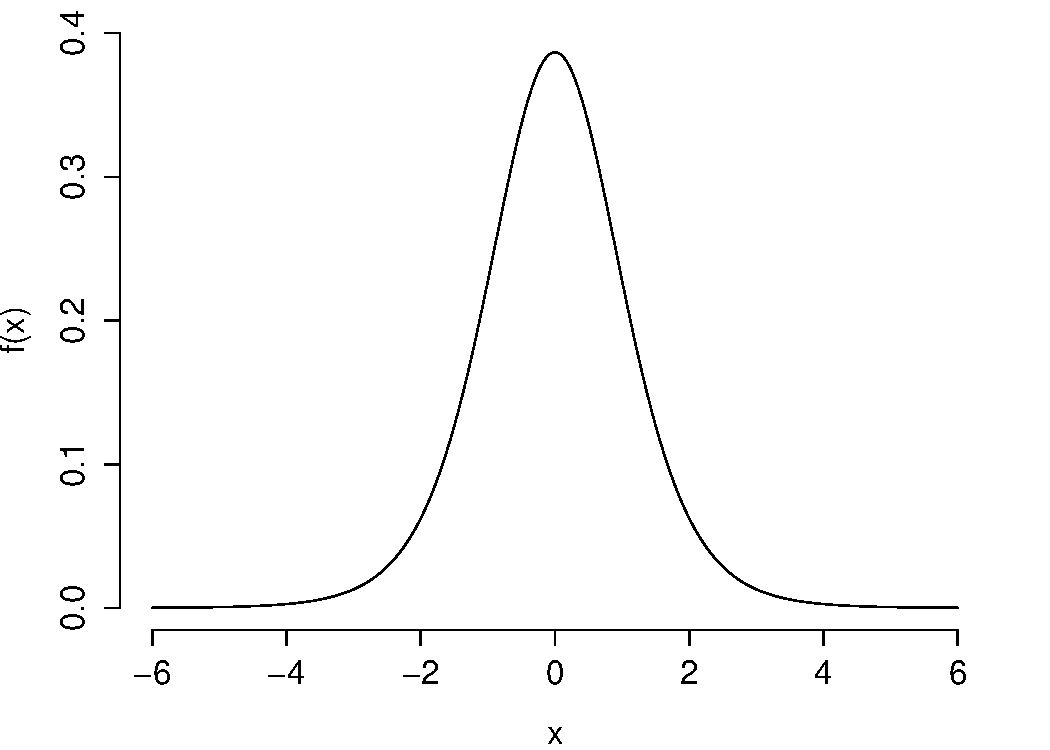
\includegraphics[scale= 0.4]{./images/p_upper1}

\end{figure}

\end{frame}

%%%%%%%%%%%%%%%%%%%%%%%%%%%%%%%%%%%%%%%%
\begin{frame}
\frametitle{What is the p-value? (One-sided Test)}
\footnotesize
Recall: p-value is \emph{smallest significance level} at which our observed test statistic would cause us to reject $H_0$. \alert{Test statistic is $1.14$. What is the one-sided p-value? }
\begin{figure}
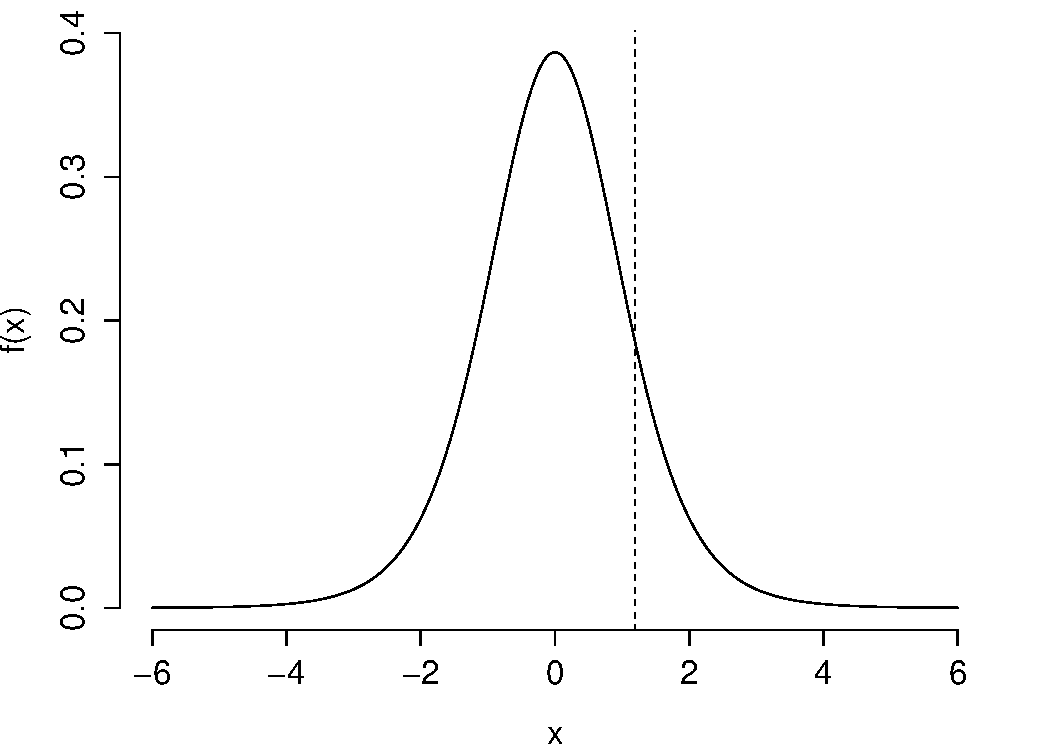
\includegraphics[scale= 0.4]{./images/p_upper2}

\end{figure}

\end{frame}

%%%%%%%%%%%%%%%%%%%%%%%%%%%%%%%%%%%%%%%%
\begin{frame}
\frametitle{What is the p-value? (One-sided Test)}
\footnotesize
Recall: p-value is \emph{smallest significance level} at which our observed test statistic would cause us to reject $H_0$. \alert{Test statistic is $1.14$. What is the one-sided p-value? }
\begin{figure}
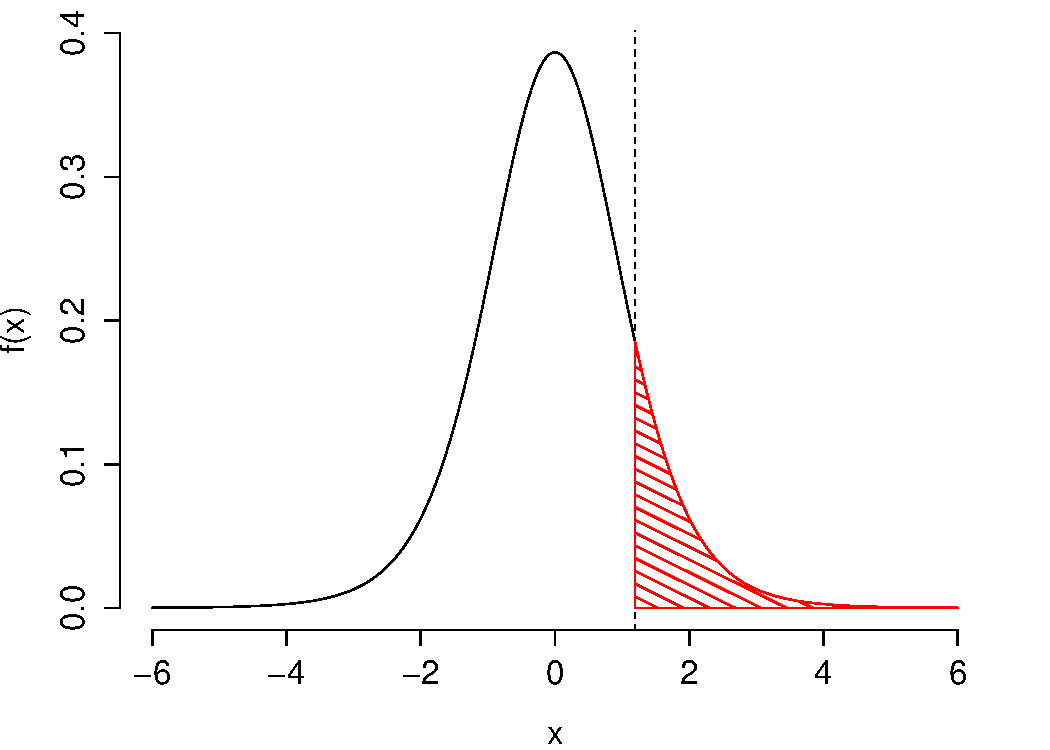
\includegraphics[scale= 0.4]{./images/p_upper3}

\end{figure}

\end{frame}

%%%%%%%%%%%%%%%%%%%%%%%%%%%%%%%%%%%%%%%%
\begin{frame}
\frametitle{What is the p-value? (One-sided Test)}
\footnotesize
Recall: p-value is \emph{smallest significance level} at which our observed test statistic would cause us to reject $H_0$. \alert{Test statistic is $1.14$. What is the one-sided p-value? }
\begin{figure}
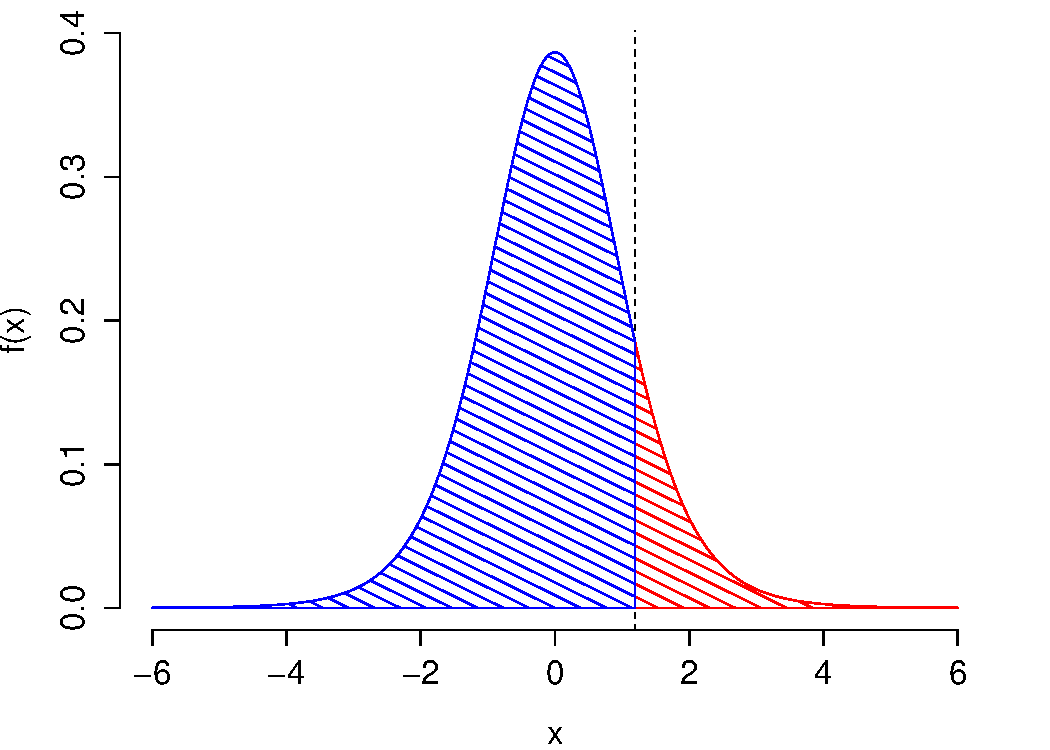
\includegraphics[scale= 0.4]{./images/p_upper4}

\end{figure}

\end{frame}

%%%%%%%%%%%%%%%%%%%%%%%%%%%%%%%%%%%%%%%%
\begin{frame}
\frametitle{What is the p-value? (One-sided Test)}
\footnotesize
Recall: p-value is \emph{smallest significance level} at which our observed test statistic would cause us to reject $H_0$. \alert{Test statistic is $1.14$. What is the one-sided p-value? }
\begin{figure}
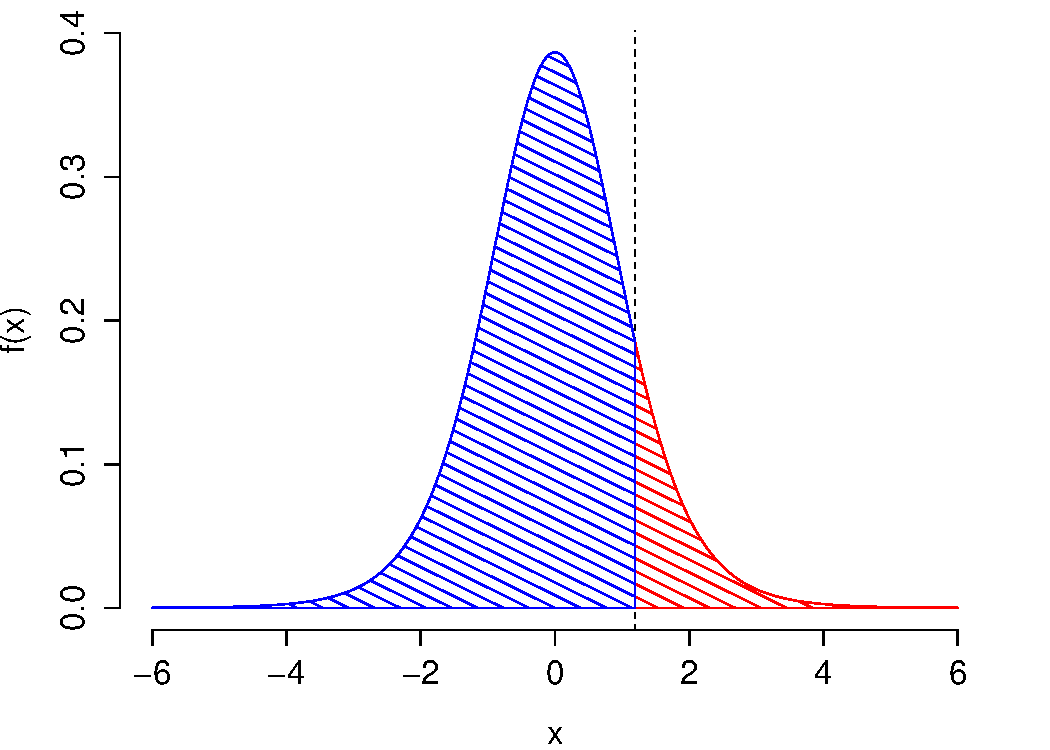
\includegraphics[scale= 0.4]{./images/p_upper4}

\end{figure}
\texttt{1 - pt(1.14, df = 8)}$\approx 0.14$
\end{frame}

%%%%%%%%%%%%%%%%%%%%%%%%%%%%%%%%%%%%%%%%
\begin{frame}
\frametitle{What is the p-value? (Two-sided Test)}
\footnotesize
Recall: p-value is \emph{smallest significance level} at which our observed test statistic would cause us to reject $H_0$. \alert{Test statistic is $1.14$. What is the two-sided p-value? }
\begin{figure}
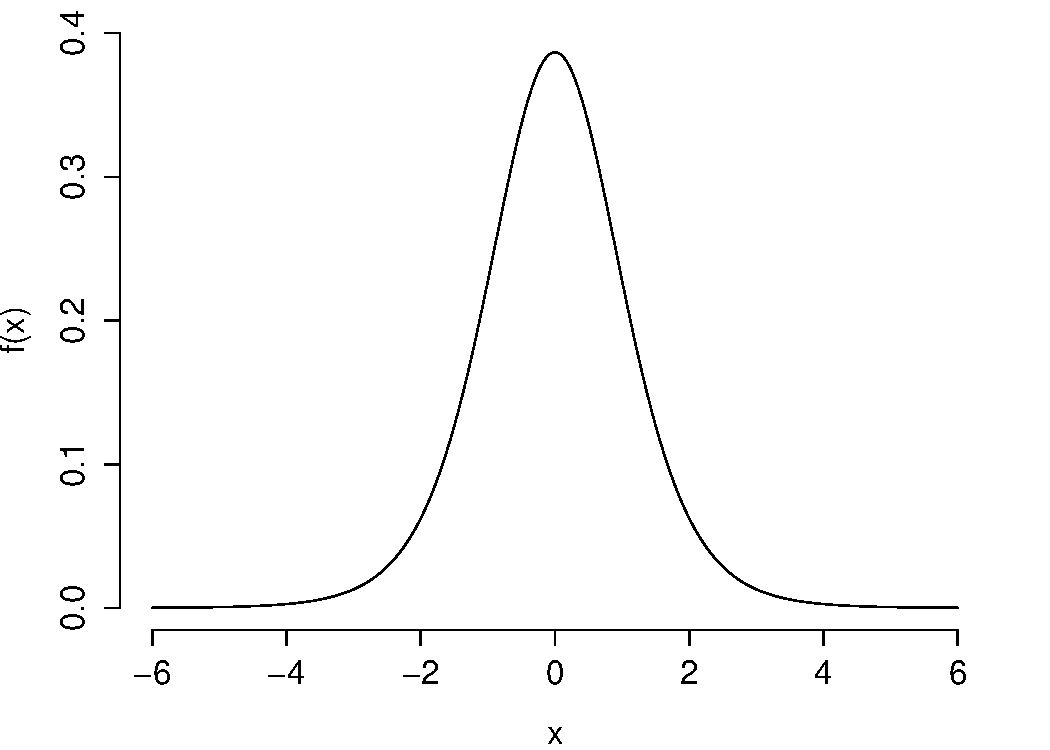
\includegraphics[scale= 0.4]{./images/p_both1}

\end{figure}

\end{frame}

%%%%%%%%%%%%%%%%%%%%%%%%%%%%%%%%%%%%%%%%
\begin{frame}
\frametitle{What is the p-value? (Two-sided Test)}
\footnotesize
Recall: p-value is \emph{smallest significance level} at which our observed test statistic would cause us to reject $H_0$. \alert{Test statistic is $1.14$. What is the two-sided p-value? }
\begin{figure}
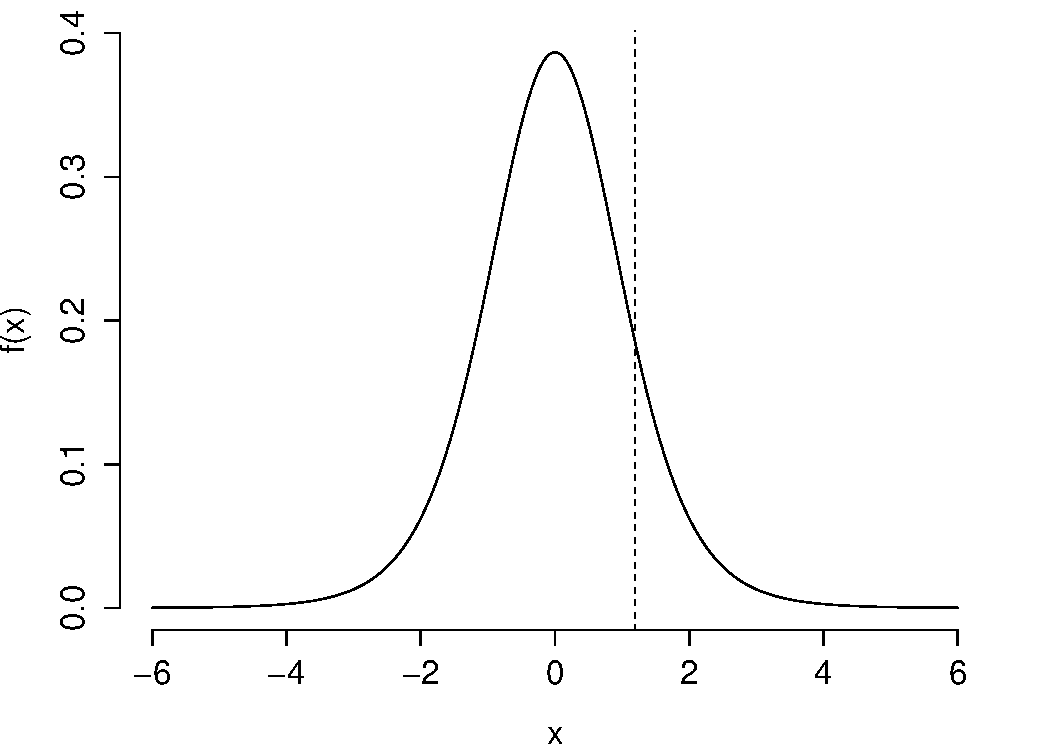
\includegraphics[scale= 0.4]{./images/p_both2}

\end{figure}

\end{frame}

%%%%%%%%%%%%%%%%%%%%%%%%%%%%%%%%%%%%%%%%
\begin{frame}
\frametitle{What is the p-value? (Two-sided Test)}
\footnotesize
Recall: p-value is \emph{smallest significance level} at which our observed test statistic would cause us to reject $H_0$. \alert{Test statistic is $1.14$. What is the two-sided p-value? }
\begin{figure}
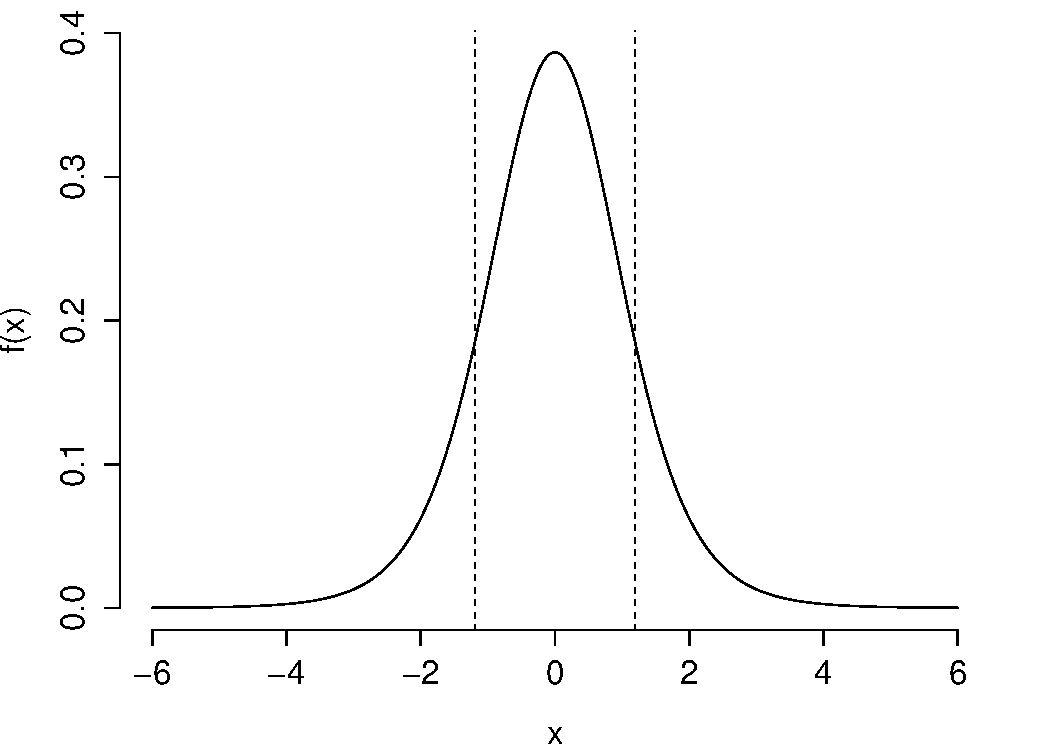
\includegraphics[scale= 0.4]{./images/p_both3}

\end{figure}

\end{frame}

%%%%%%%%%%%%%%%%%%%%%%%%%%%%%%%%%%%%%%%%
\begin{frame}
\frametitle{What is the p-value? (Two-sided Test)}
\footnotesize
Recall: p-value is \emph{smallest significance level} at which our observed test statistic would cause us to reject $H_0$. \alert{Test statistic is $1.14$. What is the two-sided p-value? }
\begin{figure}
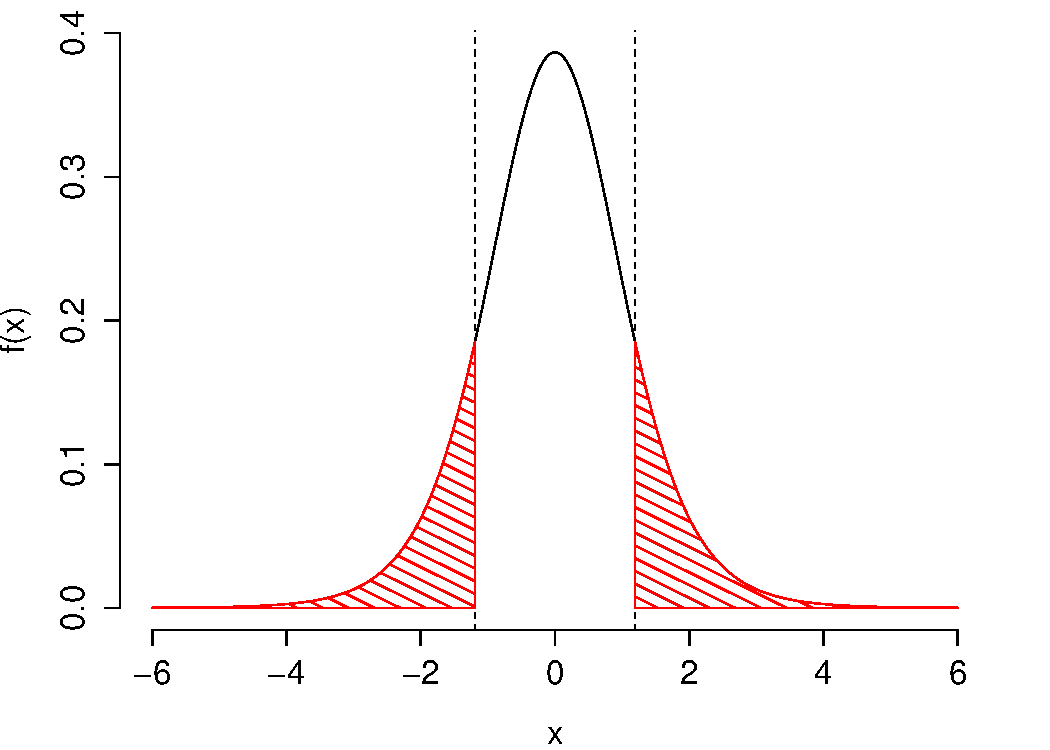
\includegraphics[scale= 0.4]{./images/p_both4}

\end{figure}

\end{frame}

%%%%%%%%%%%%%%%%%%%%%%%%%%%%%%%%%%%%%%%%
\begin{frame}
\frametitle{What is the p-value? (Two-sided Test)}
\footnotesize
Recall: p-value is \emph{smallest significance level} at which our observed test statistic would cause us to reject $H_0$. \alert{Test statistic is $1.14$. What is the two-sided p-value? }
\begin{figure}
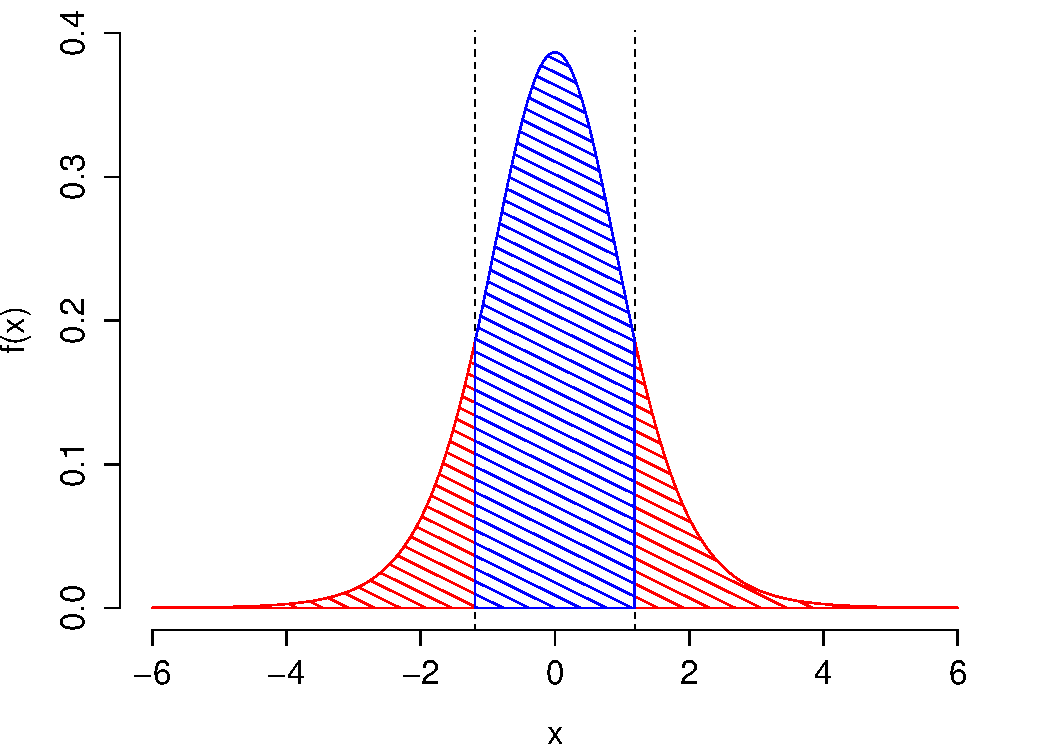
\includegraphics[scale= 0.4]{./images/p_both5}

\end{figure}

\end{frame}

%%%%%%%%%%%%%%%%%%%%%%%%%%%%%%%%%%%%%%%%
\begin{frame}
\frametitle{What is the p-value? (Two-sided Test)}
\footnotesize
Recall: p-value is \emph{smallest significance level} at which our observed test statistic would cause us to reject $H_0$. \alert{Test statistic is $1.14$. What is the two-sided p-value? }
\begin{figure}
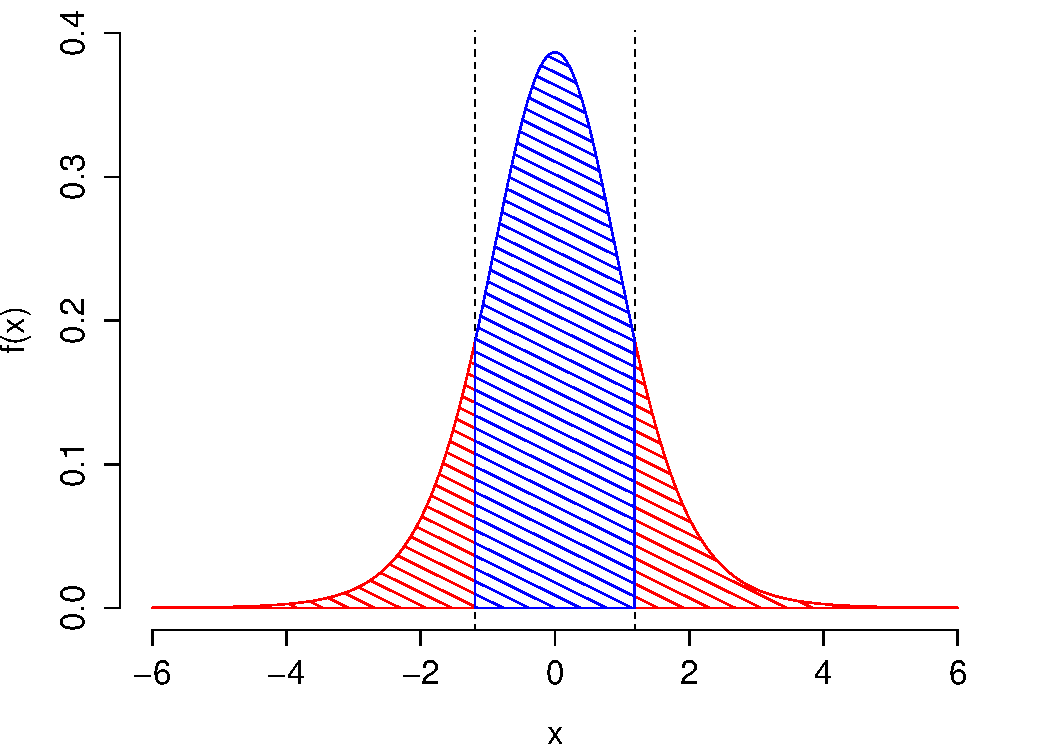
\includegraphics[scale= 0.4]{./images/p_both5}
\end{figure}

\texttt{2 * pt(-1.14, df = 8)}$\approx 0.28$ \pause \hfill \alert{This is twice the one-sided p-value!}
\end{frame}

%%%%%%%%%%%%%%%%%%%%%%%%%%%%%%%%%%%%%%%%

\begin{frame}
\frametitle{Two-sided Test is More Stringent}
\begin{block}{P-value measures strength of evidence against $H_0$}
Lower p-value means stronger evidence. 
\end{block}

\begin{block}{(Two-sided p-value) $= 2 \; \times$  (one-sided p-value)}
Reject $H_0$ based on two-sided test $\implies$ Reject $H_0$ based on appropriate one-sided test. The converse is \emph{false}.
\end{block}


\end{frame}
%%%%%%%%%%%%%%%%%%%%%%%%%%%%%%%%%%%%%%%%

\begin{frame}
\frametitle{Steps in Hypothesis Testing}

\begin{enumerate}
\item Specify Null and Alternative Hypotheses
\item Identify a Test Statistic: a function of the data that has a known sampling distribution under the null.
\item Specify a Decision Rule and a Critical Value so the Type I Error Rate equals $\alpha$.
\end{enumerate}

\begin{alertblock}{Alternative to Step 3}
	Calculate P-Value: the minimum significance level  ($\alpha$) at which we would reject $H_0$ given the observed data.
\end{alertblock}

\end{frame}


%%%%%%%%%%%%%%%%%%%%%%%%%%%%%%%%%%%%%%%%
\begin{frame}
\frametitle{How to Handle Other Examples?}

\alert{You already know lots of sampling distributions! Testing is very similar to constructing confidence intervals in that the steps are always the same, and the only thing that differs is \emph{which} sampling distribution we work with. We'll look at more examples next time.}

\end{frame}


\end{document}
